\item Considerar las transformaciones lineales $R_{\frac{\pi}{2}},S_Y,H_2$ y $P_X$ del ejercicio 11 de la práctica 2 y escribir su representación matricial con respecto a la base $B=\{(1,1),(1,-1)\}$
    \begin{mdframed}[style=s]
        \begin{itemize}
            \item $R_\frac{\pi}{2}(x,y)=(-y,x)$
                \begin{center}
                    $[R_\frac{\pi}{2}]_B=\left([R_\frac{\pi}{2}(1,1)]_B\quad[R_\frac{\pi}{2}(1,-1)]_B\right)$\\
                    $\to [R_\frac{\pi}{2}]_B=\begin{pmatrix}
                        0&1\\-1&0
                    \end{pmatrix}$
                \end{center}
                Si tomamos un vector arbitrario de $\R^2$, la transformación lo afecta de la siguiente manera
                \[[R_\frac{\pi}{2}]_B[v]_B=\begin{pmatrix}
                    0&1\\-1&0
                \end{pmatrix}\begin{pmatrix}
                    \alpha\\\beta
                \end{pmatrix}=\begin{pmatrix}
                    -\beta\\\alpha
                \end{pmatrix}\]
                En la Figura 1 se observa la transformación de dos vectores.
                \begin{center}
                    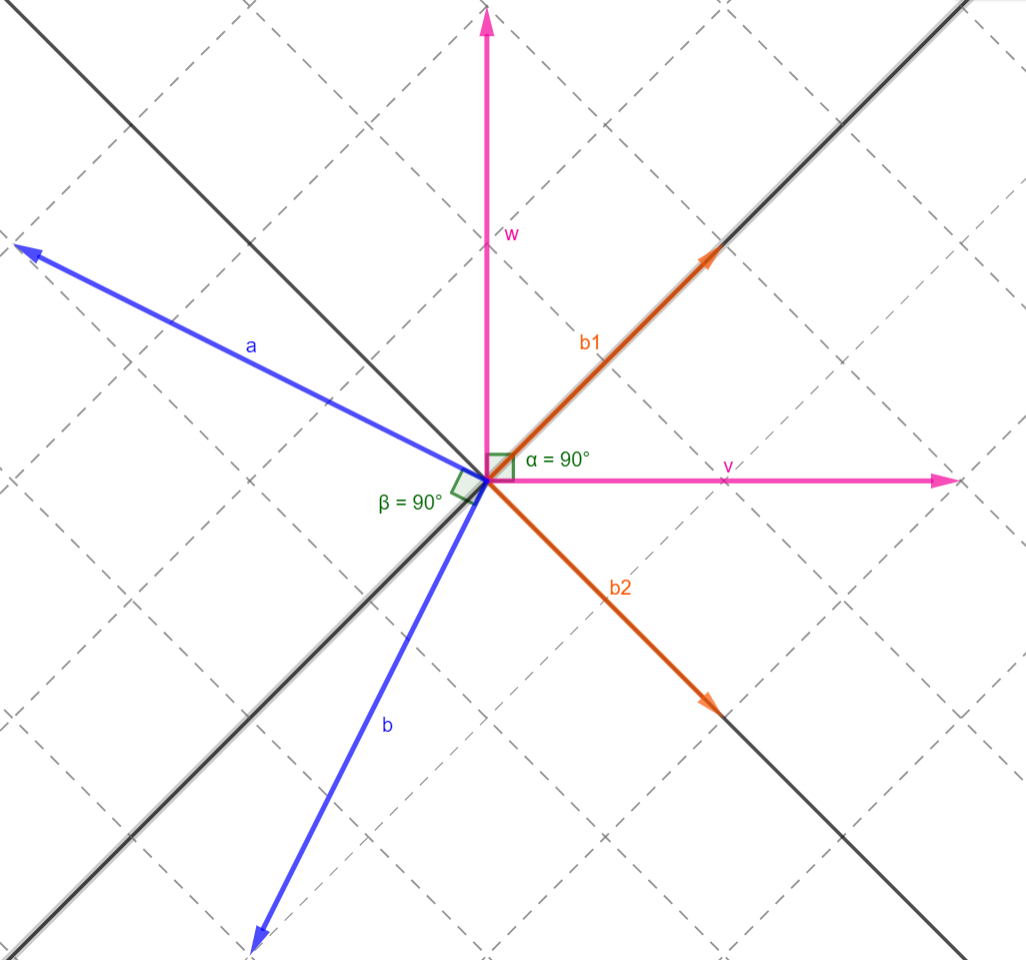
\includegraphics[width=0.4\textwidth]{Img/Ej1a.png}\\
                    Figura 1. Transformación bajo $R_\frac{\pi}{2}$ de $v$ y $a$ en el sistema de coordenadas $B$.
                \end{center}
            \item $S_Y(x,y)=(-x,y)$
                \begin{center}
                    $[S_Y]_B=\left([S_Y(1,1)]_B\quad[S_Y(1,-1)]_B\right)$\\
                    $\to [S_Y]_B=\begin{pmatrix}
                        0&-1\\-1&0
                    \end{pmatrix}$
                \end{center}
                En la Figura 2 se observan las transformaciones de los mismos dos vectores de la Figura 1, ahora bajo $S_Y$
                \begin{center}
                    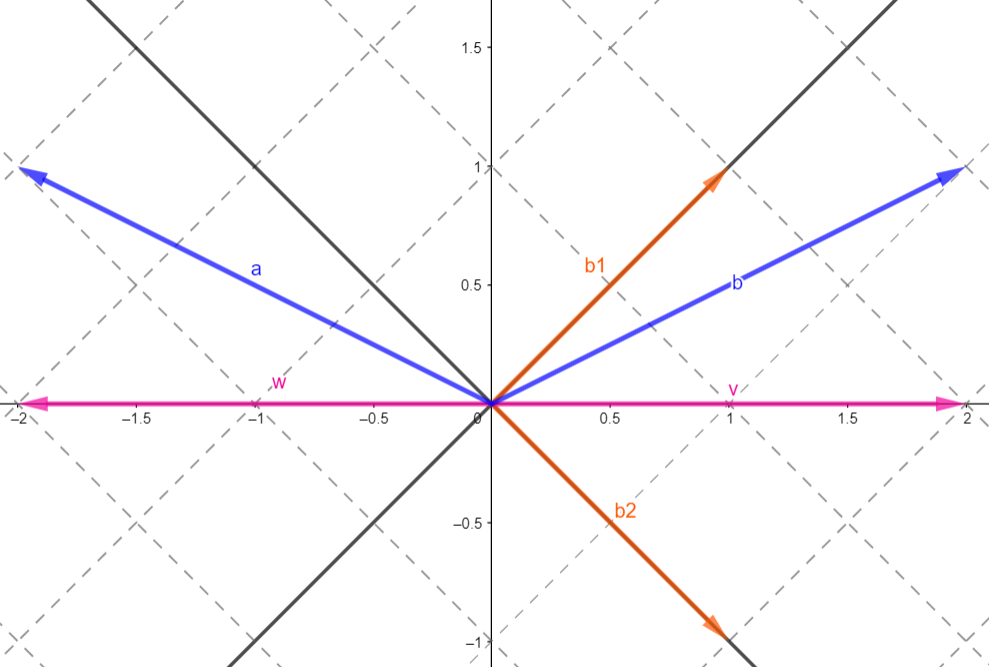
\includegraphics[width=0.4\textwidth]{Img/Ej1a2.png}\\
                    Figura 2. Transformación bajo $S_Y$ de $v$ y $a$ en el sistema de coordenadas $B$.
                \end{center}
            \item $H_2(x,y)=(2x,2y)$
                \begin{center}
                    $[H_2]_B=\left([H_2(1,1)]_B\quad[H_2(1,-1)]_B\right)$\\
                    $\to [H_2]_B=\begin{pmatrix}
                        2&0\\0&2
                    \end{pmatrix}$
                \end{center}
                En la Figura 3, se observa esta transformación.
                \begin{center}
                    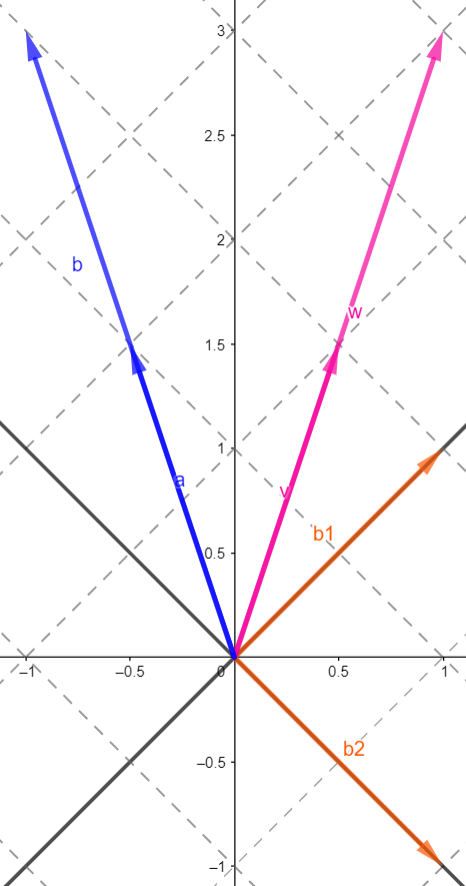
\includegraphics[width=0.2\textwidth]{Img/Ej1a3.png}\\
                    Figura 3. Transformación bajo $H_2$ de $v$ y $a$ en el sistema de coordenadas $B$.
                \end{center}
                Un dato a tener en cuenta es que \[[H_2]_B=\begin{pmatrix}
                    2&0\\0&2
                \end{pmatrix}=[H_2]_\E\]
                Supongamos el caso de la transformación más general: $H_k$ y supongamos una base cualquiera de $\R^2$, denominada $\tilde{B}=\{b_1,b_2\}$. Si quiero encontrar la representación matricial de $H_k$ en la base $\tilde{B}$:\[[H_k]_{\tilde{B}}=\left([H_k(b1)]_{\tilde{B}}\quad[H_k]_{\tilde{B}}\right)=\left([kb_1]_{\tilde{B}}\quad[kb_2]_{\tilde{B}}\right)=\begin{pmatrix}
                    k&0\\0&k
                \end{pmatrix}\]
                Por lo tanto, la representación matricial en cualquier base es la misma.¿Se puede sacar alguna conclusión de esto?
            \item $P_X(x,y)=(x,0)$
                \begin{center}
                    $[P_X]_B=\left([P_X(1,1)]_B\quad[P_X(1,-1)]_B\right)$\\
                    $\to [P_X]_B=\begin{pmatrix}
                        1/2&1/2\\1/2&1/2
                    \end{pmatrix}$
                \end{center}
        \end{itemize}
    \end{mdframed}